

Η εύρεση των πηγών ρύπων εσωτερικού αέρα είναι ένα σημαντικό κομμάτι της μελέτης της ποιότητας αέρα, για την καλύτερη αντιμετώπιση του προβλήματος. 
Πολλές φορές το πρόβλημα προσεγγίζεται με κάποιες γνωστές και συμφωνημένες συμπεριφορές που προκαλούν ρύπους, όπως είναι το κάπνισμα, το μαγείρεμα, η καύση σε εσωτερικό χώρο, η ύπαρξη ανθρώπων μες στο χώρο και η χρήση καθαριστικών προϊόντων. 
Αλλά αυτή η γνώση βασίζεται σε πάρα πολλές προηγούμενες μελέτες που έχουν γίνει.

\subsection{Πηγές ρύπων που μπορούν να βρεθούν}
Γενικά, έρευνες έχουν καταδείξει σαν κύριες πηγές ρύπου αερίων σωματιδίων και πτητικών οργανικών ουσιών στον εσωτερικό χώρο τις παρακάτω\cite{SARAGA2023165744}:


\begin {enumerate}

\item Τα υλικά κατασκευής του ίδιου του κτηρίου, με την εκπομπή αερίων τους να έχει βρεθεί από έρευνες σαν και η κύρια αιτία παραγωγής του συνόλου των πτητικών χημικών ουσιών (TVOC) στον εσωτερικό χώρος \cite{GUO20112280}.
Αυτό είναι ιδιαιτέρως αισθητό στα κτήρια που έχουν κατασκευαστεί, σε διάστημα δύο χρόνων ή έχουν ανακαινιστεί.

\item Τα έπιπλα, ειδικά τα ξύλινα έπιπλα, καθώς χρησιμοποιείται  στα ξύλινα προϊόντα μεθανάλη ή φορμαλδεΰδη (formaldehyde),η οποία μπορεί να είναι καρκινογόνα για τους ανθρώπους \cite{Salthammer2010}.

\item Οι καύσεις που γίνονται σε εσωτερικό χώρο, με λίγο κάτω από τις μισές περιπτώσεις να σχετίζονται με κάπνισμα, και μετέπειτα να βρίσκονται ξύλο, ξυλάνθρακας και κηροζίνη για μαγείρεμα και θέρμανση.
\item Πιο συγκεκριμένα, ρύποι που προέρχονται από διάφορους τρόπους μαγειρέματος, όπως είναι το ψήσιμο στην σχάρα, το τηγάνισμα και η τοστιέρα. 
Η κύρια κατηγορία ρύπων είναι τα αιωρούμενα σωματίδια σε διάμετρο κάτω των 2.5 μικρό μέτρων και των εξαιρετικά μικρών σωματιδίων (Ultra Fine Particles, UFP) .
\item Η επαναιώρηση σωματιδίων από ανθρώπινη δραστηριότητα. Ειδικά για την ορυκτή σκόνη, εισάγεται στο εσωτερικό περιβάλλον είτε μέσω  διείσδυσης στο κτήριο από τον ατμοσφαιρικό αέρα, είτε αν μεταφερθεί από ανθρώπους, έχοντας κολλήσει σε παπούτσια και ρούχα.
\item Καθαριστικά και άλλα καταναλωτικά προϊόντα. Είτε αναλύονται έως ξεχωριστές, διακριτές πηγές, είτε μπαίνουν σε μια κοινή κατηγορία έως εκπομπές προϊόντων σπιτιού.
\item Η ύπαρξη πτητικών χημικών ουσιών, μαζί με την διείσδυση Όζοντος (O3) και οξειδωτικών ριζών, προκαλεί χημικές αντιδράσεις στην ατμόσφαιρα που δημιουργούν οξυγονούχες πτητικές οργανικές ενώσεις και οργανικά αιωρούμενα σωματίδια.
 Αυτού του είδους πηγής ονομάζεται δευτερεύουσα πηγή, καθώς οι ρύποι αυτοί δημιουργούνται από την χημική αντίδραση υπαρχόντων ρύπων στην ατμόσφαιρα και δεν εκπέμπονται στον αέρα από κάποια στερεά ή υγρή μορφή, οι οποίες λέγονται πρωτογενείς ρύποι
\item Η εισαγωγή από την εξαέρωση με τον ατμοσφαιρικό αέρα ή με την διείσδυση ρύπων, ακόμα και με κλειστά παράθυρα και εξώπορτες. 
Συνήθως μπορούμε να αναγνωρίσουμε έως πηγές αιωρούμενων σωματιδίων εξωτερικής προέλευσης τις εκπομπές οχημάτων, πηγές σχετιζόμενες με την καύση, βιομηχανικές εκπομπές, μεταφορά από μεγάλες αποστάσεις, πηγές φλοιϊκής προέλευσης ή ορυκτή σκόνη,
δευτερογενές πηγές και θαλάσσιο αλάτι. Η επιρροή των σωματιδίων από τον ατμοσφαιρικό αέρα ονομάζεται λόγος εσωτερικού με εξωτερικού. 
\item Και διαφορετικά άλλες μικρότερες κατηγορίες.
\end{enumerate}


\begin{figure}[!htbp]
    \centering
    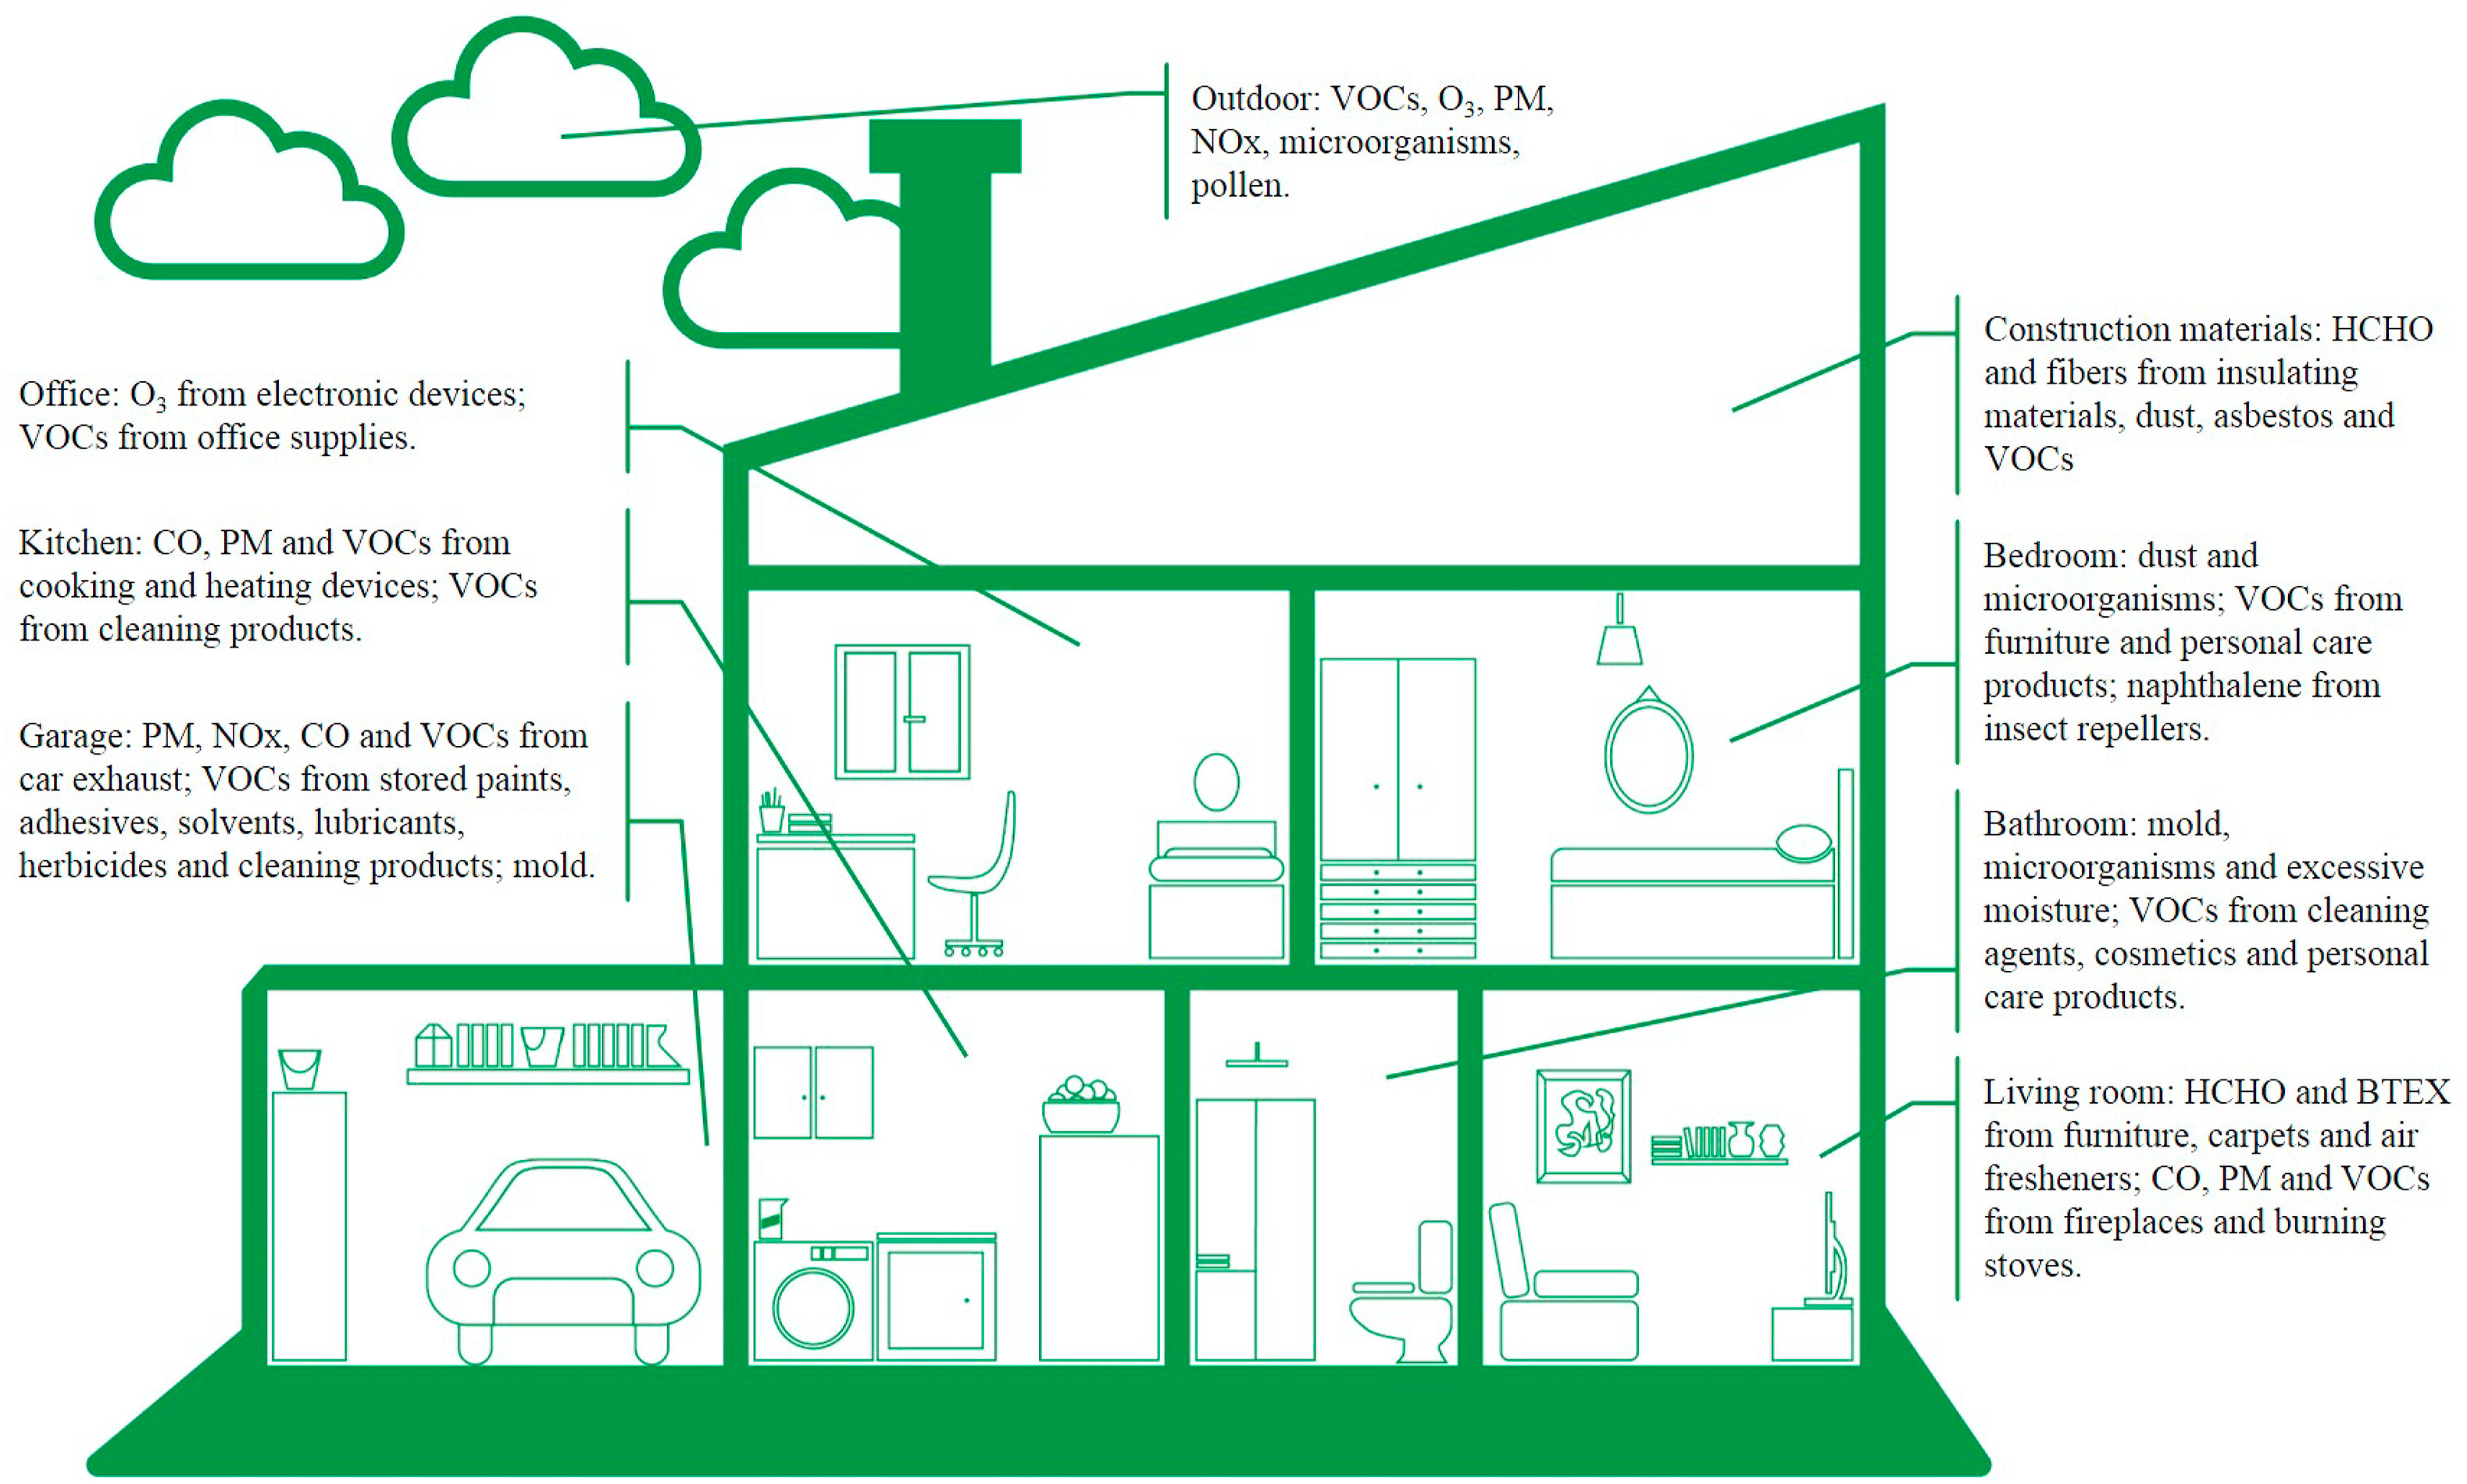
\includegraphics[width=0.8\textwidth]{εικόνες/house more common pollutants.jpg}
    \caption {Ρύποι που βρίσκονται μέσα σε ένα σπίτι και πιθανές πηγές τους \cite{GONZALEZMARTIN2021128376}}
    \label{fig:IAQ HOUSE}
\end{figure}

\FloatBarrier


\subsection{Δυσκολίες αναγνώρισης πηγών στον αέρα εσωτερικού χώρου}

Αντίθετα με τον αναγνώριση πηγών ρύπανσης στον εξωτερικό αέρα, η οποία θεωρείται σχετικά ώριμο πεδίο \cite{HOPKE2020140091}, η αναγνώριση πηγών ρύπανσης στον εσωτερικό αέρα αποτελεί ένα εξελισσόμενο πεδίο, 
καθώς παραμένει δύσκολο να προσαρμοστεί η ήδη αποκληθείσα γνώση από την μελέτη του ατμοσφαιρικού αέρα στη μελέτη του του αέρα εσωτερικού περιβάλλοντος.

Παρατηρούνται αρκετές ομοιότητες μεταξύ της, κυρίως όσον αφορά τις αρχές και τις μεθόδους που χρησιμοποιούνται και στις δύο περιπτώσεις. Επιπλέον, η εμπειρία από τη αναγνώριση πηγών στον εξωτερικό αέρα παρέχει πληροφορίες για συνήθη προφίλ πηγών εκπομπών,
τα οποία μπορούν να βοηθήσουν στον εντοπισμό πιθανών εσωτερικών πηγών και των σχετικών ιχνηθετών τους στοιχείων.

Ωστόσο, στον εσωτερικό αέρα υπάρχουν αρκετές σημαντικές διαφορές που περιορίζουν την ακρίβεια των μοντέλων αναγνώρισης των πηγών ρύπων, δυσχεραίνοντας και την ίδια την αναγνώριση τους\cite{SARAGA2024117821}.Αυτές οι διαφορές είναι:

\begin{enumerate}
    \item Οι μεγαλύτερες χωρικές και χρονικές διακυμάνσεις των συγκεντρώσεων στον εσωτερικό αέρα.
    \item Η μεγάλη ποικιλία των εσωτερικών πηγών μεταξύ ατόμων και κτιρίων
    \item Η έλλειψη ολοκληρωμένων μητρώων εκπομπών για τους ρύπους του εσωτερικού αέρα, όπως μητρώα εκπομπών για αιωρούμενα σωματίδια Ή πτητικές οργανικές ενώσεις, 
    ενώ σε ορισμένες περιπτώσεις η ίδια ιχνηθετική ουσία αντιστοιχεί σε περισσότερες από μία πηγές \cite{Bai2022}.
    \item Οι οξειδωτικές αντιδράσεις που συμβαίνουν στις επιφάνειες του εσωτερικό χώρο,
    καθώς και η θερμική διάσπαση των αερολυμάτων, δηλαδή το μείγμα του αέρα με τα αιωρούμενα σωματίδια, οδηγώντας έτσι στη δημιουργία δευτερογενών ρύπων πρώτης και δεύτερης γενιάς \cite{Morrison2019956}.
    \item Οι μηχανισμοί εξαερισμού και διείσδυσης εξωτερικού αέρα, οι οποίοι μπορούν να επηρεάσουν σημαντικά τη διανομή και τη συγκέντρωση των ρύπων \cite{Trompetter2018164}.
    Για παράδειγμα, η διείσδυση ατμοσφαιρικών οξειδωτικών, όπως η διείσδυση εξωτερικού όζοντος (O3), ή η ενδογενής παραγωγή τους μπορεί να οδηγήσει σε πολύπλοκες οξειδωτικές αντιδράσεις με τις πτητικές οργανικές ενώσεις,
    παράγοντας μεγάλη ποικιλία δευτερογενών αερίων ρύπων και αερολυμάτων \cite{Nazaroff2022}.
    \item Η διαφορά θερμοκρασίας μεταξύ του εξωτερικού αέρα και του εσωτερικού αέρα μπορεί να προκαλέσει αλλαγές φάσης συγκεκριμένων ρύπων.
    Ένα χαρακτηριστικό παράδειγμα είναι το νιτρικό αμμώνιο, το οποίο μπορεί το χειμώνα να είναι σταθερό στις εξωτερικές θερμοκρασίες, αλλά να διασπάται σε αέρινο νιτρικό οξύ και αμμωνία όταν διεισδύει,
    τα οποία με τη σειρά τους μπορεί να αλληλοεπιδράσουν με άλλους ρύπους \cite{Lunden20035633}.
    \item Οι βιολογικοί και οι αλλεργιογόνοι παράγοντες που υπάρχουν στον εσωτερικό χώρο, η κατανόηση των πηγών τους και των αλληλεπιδράσεών τους με τους χημικούς ρύπους αποτελεί ένα αναδυόμενο πεδίο έρευνας.

\end {enumerate}

\subsection{Κατηγορίες εύρεσης των πηγών ρύπων στο εσωτερικό χώρο}


\begin{enumerate}
\item  Η πιο συχνή σε έρευνες που χρησιμοποιούν LCS και IoT είναι η παρακολούθηση της ποιότητας του εσωτερικού αέρα και εξαγωγή συμπερασμάτων από τα αποτελέσματα που συγκεντρώθηκαν, συγκρίνοντας τις με τις γνώσεις που έχουμε για το τι συναίβει τις ώρες αυτές.
Ένα πολύ καλό παράδειγμα δίνεται στην έρευνα \cite{Becerra2020}.
\item Προσέγγιση επιμερισμού πηγών(Source Apportionment),που θα μιλήσουμε αναλυτικά στην συνέχεια.

\item Χρήση αντίστροφων μεθόδου χρησιμοποιώντας προσομοιώσεις Computational fluid Dynamics ή multi-zone models για την παραγωγή των δεδομένων \cite{Li2022},\cite{Liu2007}.
Έχουν χρησιμοποιηθεί σε μικρότερα βαθμό και νευρωνικά μοντέλα \cite{bastani2012}.
\item Χρήση ρομπότ με ενσωματωμένους αισθητήρες \cite{Xiao2025}

 \end {enumerate}   

\subsection{Επιμερισμός ρύπων (Source Apportionment)}

Η  εξαγωγή πληροφοριών σχετικά με τις πηγές που εκπέμπουν ρύπους του αέρα και την συμβολή της εκάστοτε πηγής στην συνολική ποιότητα του αέρα ορίζεται έως επιμερισμός ή αναγνώριση πηγών (Source Apportionment, SA).
Συμπεριλαμβάνει μια ευρεία γκάμα τεχνικών που χρησιμοποιούνται για να αποκτήσουμε γνώση σχετικά με την επίδραση που έχουν μία ή οι περισσότερες πηγές σε μία συγκεκριμένη περιοχή σε ένα συγκεκριμένο χρονικό διάστημα.
Υπάρχουν δύο κατηγορίες μοντέλων, τα μοντέλα προσαρμοσμένα στην πηγή (source-oriented  method) και τα μοντέλα προσαρμοσμένα στον υποδοχέα (receptor methods) \cite{SARAGA2023165744}.

Τα μοντέλα προσανατολισμένα στην πηγή (source-oriented models) μιμούνται τις φυσικές και χημικές διεργασίες που εμπλέκονται στην εκπομπή ρύπων. 
Χρησιμοποιούν μητρώα εκπομπών (emissions inventories) ως δεδομένα εισόδου και αξιολογούνται μέσω μοντέλων χημείας, μεταφοράς και διασποράς, για παράδειγμα συσχετίζοντας την κατεύθυνση του ανέμου με τα επίπεδα των μετρούμενων ρύπων για τον εντοπισμό των πηγών.
 Τα μητρώα εκπομπών αναπτύσσονται χρησιμοποιώντας όργανα παρακολούθησης αναφοράς (reference-grade monitoring instruments), για διάφορες πηγές ρύπων και σε πολλές τοποθεσίες.
 
 Ωστόσο, αυτά τα μητρώα μπορεί να παρουσιάζουν διαφορές στην ακρίβεια και τη συνοχή τους και συχνά δεν είναι διαθέσιμα. Κατά συνέπεια, αυτή η μέθοδος για την κατανόηση της συνεισφοράς των διαφόρων πηγών στα επίπεδα των ρύπων στον αέρα 
  μπορεί να έχει περιορισμένη εφαρμοσιμότητα \cite{Higgins2024}. Επίσης υπάρχει η ανάγκη προηγούμενης πληροφορίες για τις πηγές που υπάρχουν στον χώρο. Επειδή ασχολούμαστε με την παρακολούθηση, δεν θα μιλήσουμε παραπάνω για αυτά τα είδη μοντέλων.

Οι μέθοδοι προσανατολισμένες στον υποδοχέα (receptor-based methods) επικεντρώνονται στα χαρακτηριστικά του περιβάλλοντος υποδοχής, για να υπολογίσουν τη συνεισφορά των πηγών στο σημείο του υποδοχέα σε συγκεκριμένο χρονικό διάστημα.
Υποθέτουν τη διατήρηση της μάζας και των ειδών μεταξύ της πηγής εκπομπών και του υποδοχέα και εντοπίζουν τις πηγές λύνοντας την εξίσωση διατήρησης μάζας. 
Τα μοντέλα προσανατολισμένα στον υποδοχέα βασίζονται σε μετρημένα δεδομένα και δεν απαιτούν πρόσθετα σύνολα δεδομένων, όπως εκπομπές, μετεωρολογικές πληροφορίες ή συγκεντρώσεις αέρα στα όρια του συστήματος.
 Όσον αφορά τη συγκέντρωση των ειδών ρύπων στον υποδοχέα, αυτά τα μοντέλα είτε χρησιμοποιούν μετρημένα δεδομένα, που μπορούν να οριστούν έως δακτυλικά αποτυπώματος» ή προφίλ πηγής, είτε προκύπτουν μέσω επαναληπτικής διαδικασίας χρησιμοποιώντας κάποια προφίλ παραγόντων.

Τα μοντέλα υποδοχέα κυμαίνονται σε ένα φάσμα όσον αφορά το πόση γνώση για τις πηγές ρύπων απαιτείται.
 Τα μοντέλα Chemical Mass Balance (CMB) απαιτούν σχεδόν πλήρη γνώση των προφίλ των πηγών, καθώς πρέπει να περιλαμβάνεται ολοκληρωμένη γνώση όλων των εκπομπών σχετικών με τον υποδοχέα για την εκτίμηση της αβεβαιότητας (Mircea et al., 2020).
  Τα μοντέλα CMB για εσωτερική ρύπανση απαιτούν συνεπώς την ταυτοποίηση όλων των πιθανών πηγών ρύπων, όπως φωτιών, δραστηριοτήτων σχετικά με το μαγείρεμα, εισβολή ρύπων από την οδική κυκλοφορία κλπ.

Τα μοντέλα πολυπαραγοντικής ανάλυσης, συμπεριλαμβανομένης της Positive Matrix Factorization (PMF) 
και της Non-Negative Matrix Factorization (NMF), δεν απαιτούν πληροφορίες για τη σύσταση των πηγών. 
Αυτά τα μοντέλα χρησιμοποιούν τις συγκεντρώσεις των ειδών ρύπων στον υποδοχέα για να επιλύσουν ένα πρόβλημα σταθμισμένης παραγοντοποίησης (Mircea et al., 2020). 
Ωστόσο, στηρίζονται και σε γνωστές πειραματικές αβεβαιότητες, οι οποίες μπορεί ή όχι να είναι διαθέσιμες για δεδομένα από αισθητήρες αέρα φτηνού κόστους.

Η ενισχυτική ή «Lenschow» προσέγγιση των μοντέλων προσανατολισμένων στον υποδοχέα χρησιμοποιεί υπολογιζόμενες διαφορές στις συγκεντρώσεις μεταξύ διαφορετικών χωρικών θέσεων για τον προσδιορισμό της συνεισφοράς των πηγών (Mircea et al., 2020).
 Αυτό έχει πιθανές εφαρμογές στη χρήση LCS για μελέτες κατανομής πηγών σε εσωτερικούς χώρους, εφόσον υπάρχει αποτελεσματική στρατηγική ανάπτυξης αισθητήρων.

Τα αποτελέσματα των μοντέλων υποδοχέα αφορούν συγκεκριμένες τοποθεσίες και χρονικά παράθυρα, και δεν υποθέτουν ούτε ότι τα προφίλ των πηγών αλλάζουν σημαντικά, ούτε ότι οι ρύποι μεταβάλλονται κατά τη μεταφορά από την πηγή στον υποδοχέα.
Οι μέθοδοι προσαρμοσμένοι στον υποδοχέα ποσοτικοποιούν την συνεισφορά από πηγών ρύπων με τον να καταμετρούν την συγκεντρώσεις τους σε συγκεκριμένα σημεία, ή υποδοχείς των ρύπων \cite{Higgins2024},\cite{Mircea2020}.



\subsection {Αναγνώριση πηγών με συνεχή παρακολούθηση και χρήση αισθητήρων αέρα φτηνού κόστους}

Τα παραπάνω μοντέλα που αναφέρθηκαν στο κομμάτι \label {sub:{Επιμερισμός ρύπων (Source Apportionment)}} μπορούν να ονομαστούν και παραδοσιακοί τρόποι προσέγγισης εντοπισμού πηγών των ρύπων, καθώς βασίζονται σε μία μετέπειτα ανάλυση των δειγμάτων σε κάποιο εργαστήριο.
 Τα τελευταία χρόνια έχει αρχίζει να εντάσσεται παραπάνω η συνεχή παρακολούθηση των ρύπων για τον εντοπισμό των πηγών σε πραγματικό χρόνο, όπου χρησιμοποιούν τις παραπάνω μεθόδους, αλλά και διαφορετικές προσεγγίσεις. 

Από τις σχετικές ανασκοπήσεις ερευνών, των Chojer et al (2024), \cite{CHOJER2024103534} και ,Higgins et al (2024),\cite{Higgins2024} σχετικά με τον εντοπισμό πηγών ρύπων, η πρώτη μελετώντας την περίοδο 2017-2022 και η δεύτερη την περίοδο 2018-2023,
μόλις 4 έρευνες από την κάθε ανασκόπηση εντοπίστηκαν να χρησιμοποιούν αισθητήρες αέρα φτηνού κόστους για τον καταμερισμό πηγών, από τις 60 έκαστος που συμπεριέλαβε κάθε ανασκόπηση.

Η πρώτη ανασκόπηση των ,Chojer et al (2024),\cite{CHOJER2024103534} αναλύει γενικά τις έρευνες που έχουν γίνει για τον εντοπισμό των πηγών την περίοδο που μελετάται, ενώ η δεύτερη ανασκόπηση, Higgins et al (2024),
\cite{Higgins2024} αναφέρει τις έρευνες που έχουν γίνει για την ποιότητα εσωτερικού αέρα χρησιμοποιώντας αισθητήρες αέρα χαμηλού κόστους. Δεν είναι όλες οι έρευνες συνεχούς παρακολούθησης με αισθητήρες χαμηλού κόστους βεβαίως, 
αφού στην ανασκόπηση του Chojer et al (2024) \cite{CHOJER2024103534} ανασκόπηση, αναφέρεται ότι 9 έρευνες βρέθηκαν να χρησιμοποιούν συνεχή παρακολούθηση, οπότε οι άλλες 5 χρησιμοποίησαν όργανα αναφοράς για την καταμέτρηση.
Η ανασκόπηση του Higgins et al (2024) \cite{Higgins2024} χ αναφέρει ότι με βάση την γνώση των συγγραφέων, πρέπει να είναι ελάχιστος ή μηδενικός ο αριθμός των ερευνών που σε προηγούμενα χρόνια επιχείρησε να εντοπίσει τις πηγές ρύπων με αισθητήρες χαμηλού κόστους.

Οι έρευνες που αναφέρονται είναι οι εξής:

\begin{enumerate}

    \item Οι Bousiotis et al \cite{BOUSIOTIS2023107907} τοποθέτησαν αισθητήρες χαμηλού κόστους (LCS) στο υπνοδωμάτιο, την κουζίνα και το γραφείο μιας κατοικίας, καθώς και εκτός του σπιτιού, και χρησιμοποίησαν PMF για την επιμερισμένη εκτίμηση των συνεισφορών των PM.
     Μέτρησαν PM1, PM2.5 και PM10 και διαπίστωσαν ότι οι υψηλότερες συγκεντρώσεις PM2.5 και PM10 καταγράφηκαν στο υπνοδωμάτιο, λόγω των δραστηριοτήτων και της παρουσίας χαλιών και μαλακών επίπλων. 
     
     Παρότι η κουζίνα παρουσίασε τις υψηλότερες αιχμές PM, το γραφείο είχε τη μεγαλύτερη συγκέντρωση PM1 λόγω του αυξημένου αερισμού του, με τη διείσδυση εξωτερικών σωματιδίων να αποτελεί σημαντικό παράγοντα. 
     Συνολικά, το μοντέλο PMF έδειξε ότι το 95\% των υπέρλεπτων σωματιδίων προερχόταν από εξωτερικές πηγές.
    
    \item Οι Ainiwaer et al \cite{AINIWAER2022119652} μέτρησαν τη συγκέντρωση PM2.5 σε οκτώ διαφορετικά ύψη σε κουζίνα και υπνοδωμάτιο κατοικίας, χρησιμοποιώντας αισθητήρες χαμηλού κόστους (LCS) με υψηλή χρονική ανάλυση.
     Η χρήση αισθητήρων σε διαφορετικά ύψη τόσο κατά τις περιόδους μαγειρέματος όσο και εκτός αυτών επέτρεψε την αναγνώριση των πηγών του PM2.5.
      
     Από τις αναφορές των ενοίκων, οι συγγραφείς διαπίστωσαν ότι δεν υπήρχε καύση θυμιάματος ούτε λειτουργία συσκευών θέρμανσης κατά την περίοδο δειγματοληψίας και κατέληξαν στο συμπέρασμα ότι το μαγείρεμα και η επαναιώρηση σκόνης 
      ήταν οι μόνες δύο σημαντικές εσωτερικές πηγές αιωρούμενων σωματιδίων. Η ανάλυση κύριων συνιστωσών (PCA) χρησιμοποιήθηκε για τον χαρακτηρισμό των προτύπων πηγών και των συνεισφορών από τα επεισόδια μαγειρέματος, 
      καθώς και για τη διάκριση της συνεισφοράς εσωτερικών έναντι εξωτερικών πηγών (από σταθμό αναφοράς) στην κατακόρυφη κατανομή του PM2.5. Καταγράφηκαν μεταβολές μεταξύ 18 μg $m^{-3} $και 28 μg $m^{-3}$ σε διαφορετικές κατακόρυφες βαθμίδες στην κουζίνα,
       υπογραμμίζοντας τη σημασία της τοποθέτησης των αισθητήρων κατά τη μέτρηση ρύπων που προέρχονται από δραστηριότητες μαγειρέματος.
    
    \item Οι Liu et al \cite{Liu2023} μέτρησαν τις συγκεντρώσεις PM2.5 σε περισσότερα από 100 νοικοκυριά και στο εξωτερικό περιβάλλον στην Κίνα, κατά τη διάρκεια περιόδου έξι μηνών, και αξιολόγησαν τις ενδοοικιακές και διαοικιακές μεταβολές του PM2.5. 
    Αρχικά, οι συγγραφείς χρησιμοποίησαν ένα μικτό μοντέλο για να εντοπίσουν τους παράγοντες που επηρεάζουν τις ενδοοικιακές και διαοικιακές μεταβολές της συγκέντρωσης PM2.5. 
    Οι ενδοοικιακοί παράγοντες που επηρέαζαν τις συγκεντρώσεις περιλάμβαναν το εξωτερικό PM2.5, την εξωτερική θερμοκρασία, την ταχύτητα και τη διεύθυνση του ανέμου, τη διαφορά θερμοκρασίας, την εποχή και τη συγκέντρωση του εσωτερικού PM2.5 της προηγούμενης ημέρας.
     Ο
     ι διαοικιακοί παράγοντες επιρροής περιλάμβαναν τον τύπο καυσίμου, τα ανοιχτά παράθυρα και τη διαφορά θερμοκρασίας, καθώς και το μορφωτικό επίπεδο και την ηλικία των κατοίκων. 
     Στη συνέχεια, οι συγγραφείς χρησιμοποίησαν μέθοδο επιμερισμού πηγών για να προσδιορίσουν τις συγκεντρώσεις PM2.5 που προέρχονταν από τρεις κύριες πηγές, τη διείσδυση από το εξωτερικό περιβάλλον, τη χρήση στερεών καυσίμων για θέρμανση ή μαγείρεμα 
     και άλλες μη προσδιορισμένες πηγές — και διαπίστωσαν ότι η καύση στερεών καυσίμων συνέβαλε κατά 31\%–55\% στο PM2.5. Τέλος, συνέστησαν την αντικατάσταση των στερεών καυσίμων με πέλλετ βιομάζας, προκειμένου να επιτευχθεί σημαντική μείωση των συγκεντρώσεων PM2.5.
    
    \item Οι Zhang et al \cite{ZHANG2022109643} αξιοποίησαν δεδομένα από το Air Quality Egg V2 καθώς και από το προσαρμοσμένο σύστημα αισθητήρων χαμηλού κόστους (LCS) που ανέπτυξαν οι ίδιοι, χρησιμοποιώντας αισθητήρες από τον ίδιο κατασκευαστή.
     Στόχος των συγγραφέων ήταν η διερεύνηση των σχέσεων μεταξύ των συγκεντρώσεων ρύπων εσωτερικού αέρα και αρχιτεκτονικών–περιβαλλοντικών χαρακτηριστικών πανεπιστημιακών κτιρίων. 
     Εφάρμοσαν ανάλυση κυρίων συνιστωσών (PCA) για τον εντοπισμό των παραγόντων που επηρεάζουν τις συγκεντρώσεις αιωρούμενων σωματιδίων (PM), διοξειδίου του αζώτου (NO2) και όζοντος (O3).

    Οι συνθήκες εσωτερικού αερισμού ήταν ελεγχόμενες σε όλα τα κτίρια και περιλάμβαναν κλιματισμό, μηχανικό αερισμό, φίλτρα HEPA με προδιαγραφή MERV13 και κλειστά παράθυρα. 
    Διαπιστώθηκαν ισχυρές συσχετίσεις μεταξύ των εσωτερικών τιμών PM2.5, PM10 και O3 και των αντίστοιχων εξωτερικών συγκεντρώσεων, καθώς και με την απόσταση του κτιρίου από κύριους οδικούς άξονες, την ύπαρξη ρωγμών στη δομή του κτιρίου, 
    την εξωτερική θερμοκρασία και την υγρασία. 
    
    Οι συγκεντρώσεις NO2 στο εσωτερικό επηρεάζονταν επίσης από την απόσταση του κτιρίου από την κύρια κυκλοφορία, καθώς και από τη σχετική υγρασία εσωτερικού χώρου, το O3 , την παρουσία γριλιών αερισμού, 
    τον όγκο του χώρου και τον λόγο επιφάνειας παραθύρων προς επιφάνεια τοίχων.
    
    \item Οι Shen et al \cite{SHEN2021145304}  χρησιμοποιήθηκαν αισθητήρες χαμηλού κόστους για τη μέτρηση των συγκεντρώσεων PM2.5 σε ένα τυπικό διαμέρισμα στο Πεκίνο.
     Διαπιστώθηκε ότι τα αιωρούμενα σωματίδια εσωτερικού χώρου προέρχονται κυρίως από τη διείσδυση του εξωτερικού αέρα και από τις εκπομπές που σχετίζονται με το μαγείρεμα, με τις τελευταίες να συμβάλλουν περισσότερο στα λεπτόκοκκα σωματίδια. 
     
     Οι συγκεντρώσεις PM2.5 στο εσωτερικό βρέθηκαν να συσχετίζονται με τα επίπεδα του εξωτερικού περιβάλλοντος, αλλά ήταν γενικά χαμηλότερες από τις εξωτερικές, με μέσο λόγο εσωτερικού/εξωτερικού (I/O) ίσο με 0,85.
    Η κυρίαρχη εσωτερική πηγή ήταν το μαγείρεμα, το οποίο προκαλούσε περιστασιακά υψηλές αιχμές συγκέντρωσης.

    Οι μεταβολές που παρατηρήθηκαν στους περισσότερους χώρους παρουσίαζαν χρονική υστέρηση σε σχέση με εκείνες που μετρήθηκαν στο εξωτερικό περιβάλλον και στην κουζίνα που μελετήθηκε. 
    Οι διαφορές μεταξύ των δωματίων διαπιστώθηκε ότι εξαρτώνται από τις αποστάσεις των διαδρομών μεταφοράς από τις πηγές.
    
    Κατά μέσο όρο, οι εξωτερικές πηγές συνέβαλαν κατά 36\% στο εσωτερικό PM2.5, με τη συνεισφορά αυτή να παρουσιάζει σημαντικές χρονικές και χωρικές διακυμάνσεις.

    \item Οι Saad et al \cite{Saad2017} προτείνει ένα ενισχυμένο σύστημα παρακολούθησης της ποιότητας εσωτερικού αέρα (IAQMS), το οποίο μπορεί να αναγνωρίζει τους ρύπους αξιοποιώντας εποπτευόμενους αλγορίθμους μηχανικής μάθησης: 
    πολυεπίπεδο perceptron (MLP), K-πλησιέστερων γειτόνων (KNN) και γραμμική διακριτική ανάλυση (LDA). 
    Δοκιμάστηκαν πέντε πηγές ρύπανσης του εσωτερικού αέρα: ατμοσφαιρικός αέρας, δραστηριότητες καύσης, παρουσία χημικών ουσιών, παρουσία αρωμάτων και παρουσία τροφίμων και ποτών.

    Τα αποτελέσματα έδειξαν ότι και οι τρεις αλγόριθμοι ταξινομούν επιτυχώς τις πέντε πηγές ρύπανσης του εσωτερικού αέρα, με ποσοστό ταξινόμησης που φτάνει έως και το 100\%. 
    Ένας ταξινομητής MLP με δομή μοντέλου 9-3-5 επιλέχθηκε για ενσωμάτωση στο παραπάνω σύστημα. Το σύστημα δοκιμάστηκε επίσης με την ταυτόχρονη παρουσία όλων των πηγών ρύπανσης του εσωτερικού αέρα. 
    Τα αποτελέσματα έδειξαν ότι το σύστημα είναι σε θέση να ταξινομεί περιπτώσεις όπου εμφανίζονται μεμονωμένες ή δύο μικτές πηγές ταυτόχρονα. Ωστόσο, όταν περισσότερες από δύο πηγές ρύπανσης του εσωτερικού αέρα εμφανίζονται την ίδια χρονική περίοδο,
     το σύστημα τις ταξινομεί ως «άγνωστες», καθώς δεν μπορεί να αναγνωρίσει την είσοδο ενός νέου προτύπου.

    \item Οι Men et al \cite{MEN2021117753} παρακολούθησαν τον εσωτερικό PM2.5 σε αγροτικές κατοικίες που χρησιμοποιούσαν άνθρακα για περίπου 4 μήνες και αναλύθηκαν η χρονική δυναμική, οι κατανομές, η σχέση με το εξωτερικό PM2.5 
    και οι ποσοτικές συνεισφορές των εσωτερικών πηγών. Διαπιστώθηκε μια διπλοκορυφική κατανομή του εσωτερικού PM2.5, με το χαρακτηριστικό της διπλής κορυφής να είναι πιο εμφανές σε πιο λεπτομερή χρονική ανάλυση. 
    Οι μέγιστες τιμές της διπλοκορυφικής κατανομής αντιστοιχούσαν στις εκπομπές από ισχυρές εσωτερικές πηγές και στη επίδραση του εξωτερικού PM2.5, αντίστοιχα.

    Το εσωτερικό PM2.5 βρέθηκε να συσχετίζεται με το εξωτερικό PM2.5, αν και η καύση άνθρακα για θέρμανση θεωρούνταν η κυρίαρχη πηγή του εσωτερικού PM2.5. Η σχέση εσωτερικού–εξωτερικού παρουσίασε 
    σημαντικές διαφορές μεταξύ της περιόδου θέρμανσης και της μη θέρμανσης. Οι επιδράσεις τυπικών εσωτερικών πηγών, όπως το μαγείρεμα, η θέρμανση με άνθρακα και το κάπνισμα, αναλύθηκαν ποσοτικά με βάση τα δεδομένα υψηλής χρονικής ανάλυσης του PM2.5.
     Η εκτιμώμενη συνεισφορά του εξωτερικού PM2.5 στο εσωτερικό ήταν περίπου 48\% κατά την περίοδο μη θέρμανσης, αλλά μειωνόταν σε περίπου 32\% κατά την περίοδο θέρμανσης. Η συνεισφορά της εσωτερικής θέρμανσης με καύση άνθρακα έφτανε έως το 47\% του εσωτερικού PM2.5 
     κατά την περίοδο θέρμανσης, ενώ οι άλλες εσωτερικές πηγές συνέβαλαν περίπου κατά 20\%.


    
\end{enumerate}
